\section{Extended fiducial phase-space study}
\label{sec:fps}

This section gives a preliminary scalar central value for an extended fiducial domain, with a three-prior
dependence envelope, a hidden-variable closure and a 200-toy containment diagnostic for the extension. The
signal remains $\nu_\mu$ CC in the tracker interaction fiducial volume. The truth-muon
kinematic cuts are removed, but the reconstructed MINOS-based selection is unchanged,
so the domain is an extended \emph{fiducial} one, not unrestricted neutrino phase space. No covariance is
quoted for it, so the result consists of central values and these validation tests.
% Accuracy fix (unscored; Joseph, DECISION-20261026-joseph-fps-scope-r04-sensitivity-and-tex-reflow.md, via the director 2026-10-26): "No corrected covariance exists for it" was
% false as read: an extended-fiducial covariance with re-selected lateral bands exists (job 56431823, 2026-08-07;
% nd-unfolding/uq_fps/corrected/FPS_UQ_CORRECTED_STATE.md:127) but is not quoted (AGENTS.md:36).
% Search: extended-fiducial covariance quoted; corrected FPS covariance; activelat (note, paper and primer closures: no
% printed extended-fiducial covariance or uncertainty beyond the three-prior envelope; AGENTS.md:36 "Old unified 4D/FPS
% covariances ... are unquotable") @ 7ad668f4
% Register pass b8 (2026-10-22): register only; every number and limitation kept (ledger.md rows F*).

\subsection{Acceptance and the extended domain}
The published cuts ($\theta_\mu<20^{\circ}$, $1.5<\pPar<\SI{60}{GeV/c}$,
$\pT<\SI{4.5}{GeV/c}$) exclude a third of the signal. Of the weighted true
$\nu_\mu$~CC rate in the tracker fiducial volume, \SI{66.4}{\percent} lies
inside the cuts, \SI{22.3}{\percent} at $\pPar<\SI{1.5}{GeV/c}$,
\SI{11.3}{\percent} at $\theta_\mu>20^{\circ}$, and the high-$\pT$/$\pPar$
tails are negligible (Fig.~\ref{fig:fpsacc}). OmniFold's treatment of events that fail reconstruction
already corrects for acceptance, so removing the truth-level kinematic cuts is a change of configuration
only: the truth denominator grows from 32.8 million to 49 million events, and the reconstruction
selection, including the MINOS match, is unchanged. In regions without acceptance the unfold extrapolates
through the step-1 regressor for missed events; the validation tests below quantify the resulting
prior dependence.

\begin{figure}[H]
  \centering
  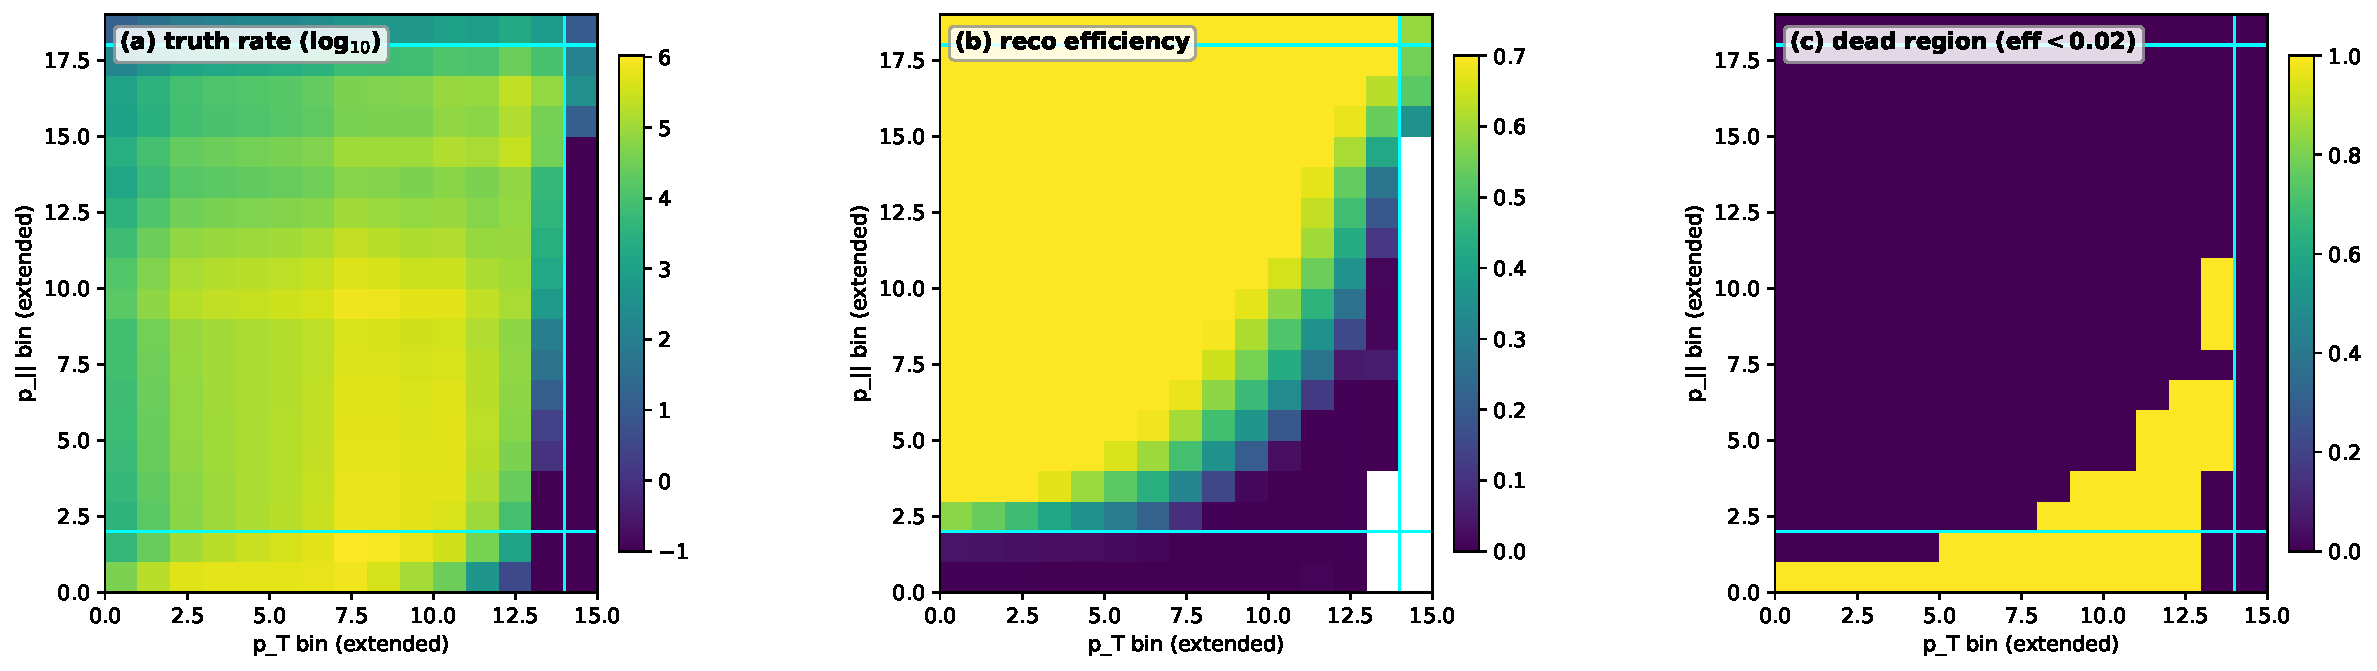
\includegraphics[width=0.99\textwidth]{fps_acceptance_MEFHC}
  \caption{Extended-fiducial acceptance across all twelve playlists:
  (a)~weighted truth rate (log$_{10}$), (b)~reconstruction efficiency, and
  (c)~the dead region with $\epsilon<\SI{2}{\percent}$, on the extended
  $(\pT,\pPar)$ grid (bin number; catch bins are too wide for a linear
  axis). Cyan lines mark the published boundary. Efficiency is
  $\sim0.65$ and flat through the published region, degrades smoothly across
  the $\theta>20^{\circ}$ wedge, and falls to zero in the $\pPar<\SI{1.5}{GeV/c}$
  strip and the high-$\pT$ corner. The dead region carries
  \SI{27.7}{\percent} of the total truth rate.}
  \label{fig:fpsacc}
\end{figure}

\subsection{Validation battery}
Four tests characterize the extension (Fig.~\ref{fig:fpscmp}):
\begin{enumerate}[itemsep=2pt]
  \item \textbf{Published-region check.} In the published sub-block, the extended unfold reproduces the control
        (standard 2D input, paper grid, identical settings) with
        integral ratio $0.9994$, median cell ratio $1.0013$, and median
        deviation \SI{\fpsAnchor}{\percent} across all 185 reported cells:
        in the published region the extended unfold agrees with the control at this level. The control's
        total, $\SI{\sigTwoDPurity}{cm^2/nucleon}$, equals at the printed precision that of the
        purity-subtracted 2D central values (exact-split and LightGBM). The quoted 2D result, with refined
        negative-weight subtraction, is $\SI{\sigTwoD}{cm^2/nucleon}$, \SI{\roFpsDiff}{\percent} lower, so the
        control no longer reproduces it.
% RE-2 integration W3 (approved, DECISION-20261024-joseph-approve-integration-wording-s1-compute-preserve.md): RE2-PARTC-REPORT.md sec. 8 (RO-FPS: E_R 3.069e-38 against the control's 3.073e-38, -0.14 %,
% "It does not reproduce"); the control: VALIDATION_LEDGER.md:1624-1625 (no committed digest; VL177 records the -0.14 %); the exact-split total
% 3.0733e-38 (values.tex \sigTwoD comment).
  \item \textbf{Closure.} Extended-grid self-closure using simulated reconstruction as
        pseudo-data returns recovered/truth $=1.0000$ in every cell,
        including the extension, with no event-accounting or normalization bias
        from the enlarged denominator. In \emph{hidden-variable} closure,
        a Gaussian truth bump is injected in true $E_{\mathrm{avail}}$,
        unseen by the $(\pT,\pPar)$ unfold. The recovered cross section
        reproduces the bump-reweighted $(\pT,\pPar)$ truth to
        median \SI{0.17}{\percent} (90th percentile \SI{0.65}{\percent}) in
        the published cells and median \SI{0.77}{\percent} (max
        \SI{4.05}{\percent}) in the extension, both well inside the prior envelope.
  \item \textbf{Three-prior envelope.} Repeating the unfold with three priors
        (MINERvA Tune~v1, bare GENIE, and NuWro-shaped) spans the
        total cross section by only $\pm\SI{1.5}{\percent}$. The NuWro-shaped
        prior reweights the truth $(\pT,\pPar)$ shape to two million raw
        NuWro events without phase-space cuts. The sample's mis-sampled flux
        (\S\ref{sec:3d-models})
        % \texttt{KNOWN\_ISSUES.md} row 83; flux repair of 2026-09-27
        suppresses its high-$\pPar$ shape, and this prior was not rebuilt after
        the flux repair. Per-cell half-spread/mean has median
        \SI{2.9}{\percent} in the published region and \SI{7.9}{\percent}
        (90th percentile \SI{62}{\percent}) in the extension, concentrated
        in zero-acceptance cells (Fig.~\ref{fig:fpsenv}).
  \item \textbf{Containment diagnostic.} With a fixed estimator seed and one 100/100 calibration--evaluation
        split, widths learned from the disjoint calibration half contain the
        fixed truth in \SI{\covFPS}{\percent} of evaluation bin--toy cells,
        compared with the \SI{\covNominal}{\percent} Gaussian nominal.
        Bin correlations and estimated widths preclude a global binomial error
        or a calibrated test. The diagnostic probes the statistical closure-toy stream, not a full uncertainty band.
        The statistical-band, pull and regional fractions are in App.~\ref{sec:fps-fractions};
        none is used as a covariance-certification test.
\end{enumerate}

\begin{figure}[H]
  \centering
  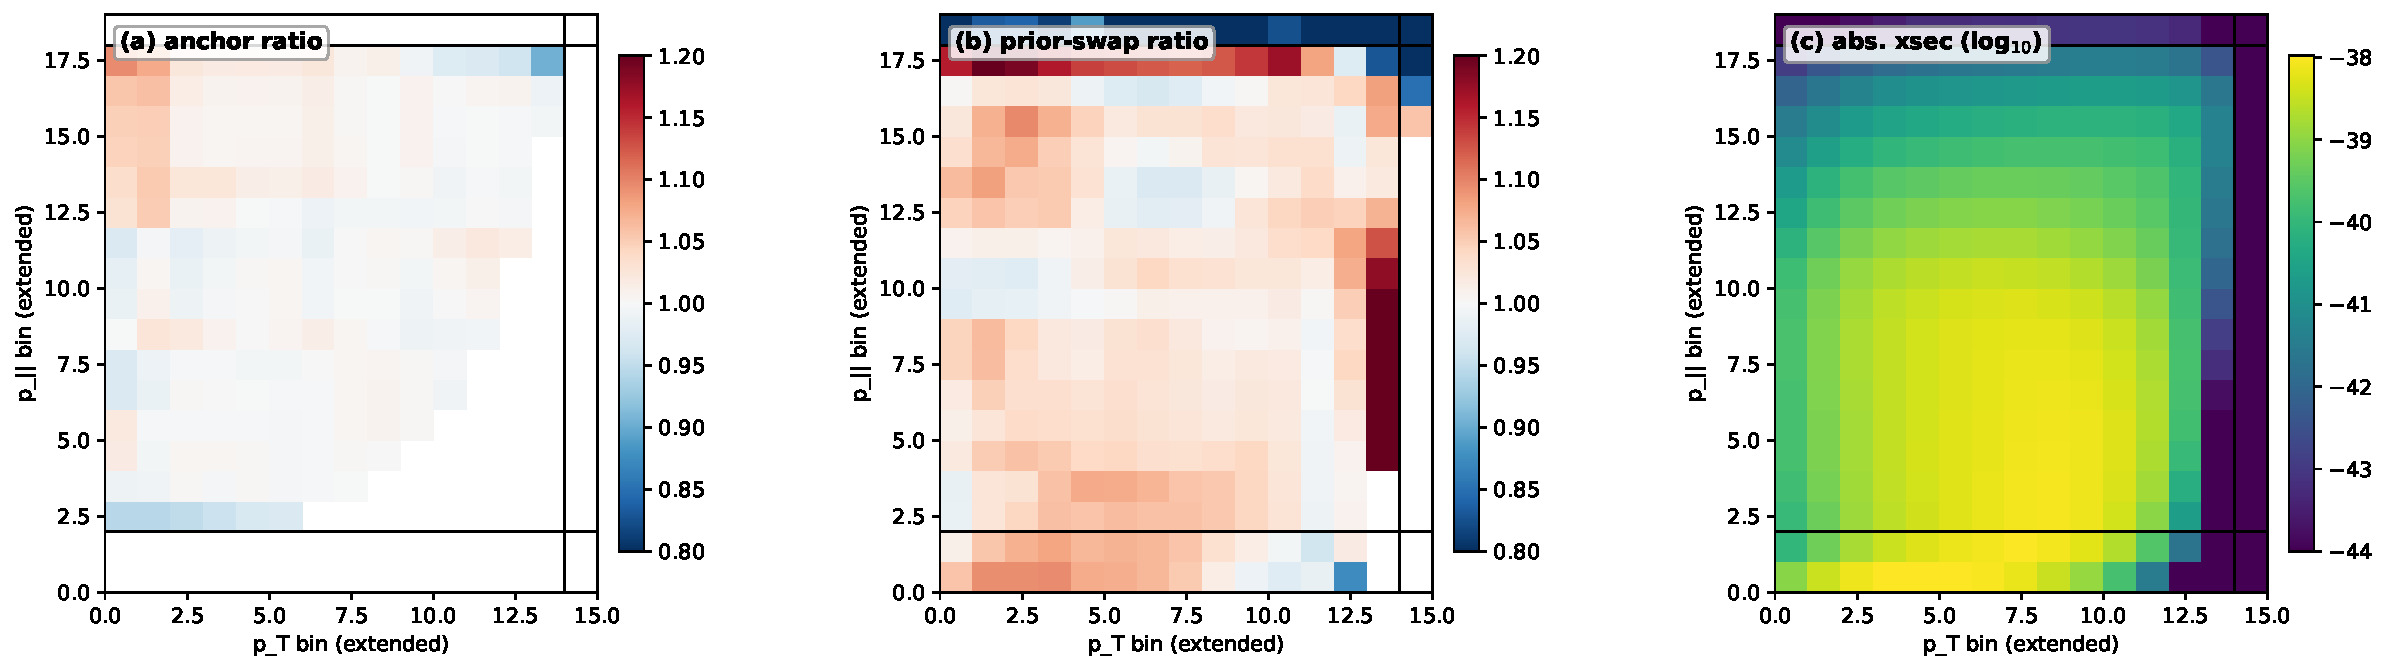
\includegraphics[width=0.99\textwidth]{fps_pilot_compare_MEFHC}
  \caption{Extended-fiducial validation battery (all playlists):
  (a)~ratio to the control in the published sub-block (median $1.0013$), (b)~MINERvA Tune~v1/bare-GENIE prior-swap ratio, and (c)~extended-fiducial
  cross section (log$_{10}$). Panels (a) and (b) are \emph{ratios} (diverging
  scale centered at unity); (c) gives \emph{absolute} magnitude on a sequential
  scale --- hence the two color schemes. Black lines mark the published
  boundary; axes are bin number on the extended grid.}
  \label{fig:fpscmp}
\end{figure}

\begin{figure}[H]
  \centering
  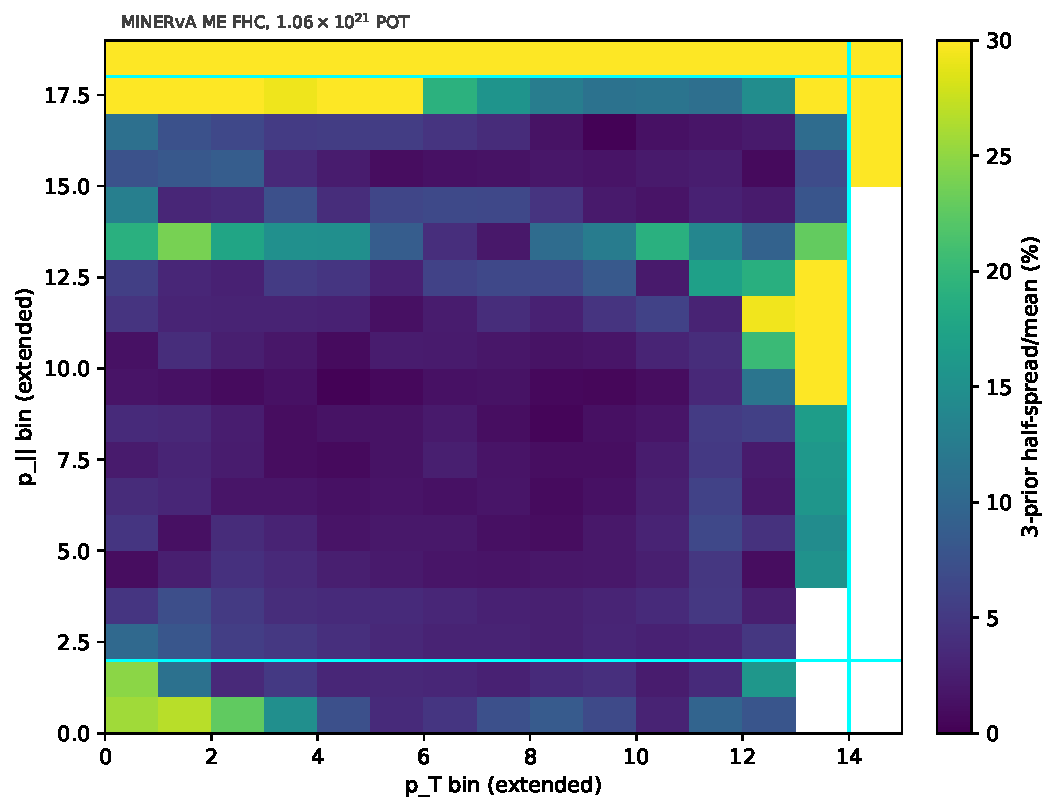
\includegraphics[width=0.62\textwidth]{fps_prior_envelope_MEFHC}
  \caption{Three-prior dependence envelope (half-spread/mean per cell,
  in percent). Prior dependence is at the few-percent level wherever the
  detector has acceptance and reaches tens of percent only in the dead
  cells --- the quantitative basis for the two-tier reporting.}
  \label{fig:fpsenv}
\end{figure}

\subsection{Central value and two-tier reporting}
The preliminary extended-fiducial CC-inclusive central value on the tracker
fiducial volume is
\begin{equation*}
  \sigma_{\mathrm{ext}} = \SI{\fpsSigma}{cm^2/nucleon}
  \quad\text{(central value)},
\end{equation*}
% RE-2 integration W5 (approved, DECISION-20261024-joseph-approve-integration-wording-s1-compute-preserve.md): \fpsAbove (46) is not printed; its definition is not established (RE2-PARTC-REPORT.md
% sec. 4: 4.502/3.0730 - 1 = 46.50 %; VALIDATION_LEDGER.md:1626 "+46% vs restricted" names no operand). The two totals:
% VALIDATION_LEDGER.md:1624-1625 (control 3.073e-38; FPS total 4.502e-38).
compared with $\SI{\sigTwoDPurity}{cm^2/nucleon}$ for the control unfold in the restricted phase
space. The extended-fiducial central value was produced with the binned purity correction (the battery of 2026-06-10), not
with refined negative-weight subtraction, the treatment designated for the extended-fiducial analysis (App.~\ref{app:negweight}).
% Accuracy fix (unscored; Joseph, DECISION-20261026-joseph-fps-scope-r04-sensitivity-and-tex-reflow.md, via the director 2026-10-26): "No extended-fiducial production with
% refined negative-weight subtraction has been run" was false as read: ten negweight-refined extended-fiducial endpoint
% unfolds were run later (job 56430128; nd-unfolding/sbatch_unfold_active_fps.sh:18,34-35,60). The sentence now says
% only what the quoted central value used, in the words of Joseph's selected option, and keeps the base sentence's fact that a
% negative-weight treatment is designated for this analysis. That treatment is refined negative-weight subtraction: App. C
% sec:negweight-footing designates negative-weight injection with Stay-Positive refinement (app_negweight.tex:370-371), the
% refined form of negative-weight injection (:257-258) whose refinement is the Stay-Positive classifier (:476) (director, 2026-10-26).
% Search: extended-fiducial central value; fps battery; 54244120; negweight-refined FPS central value (app_provenance.tex
% fps-battery; no refined extended-fiducial central value is recorded; sbatch_unfold_active_fps.sh:67 takes the existing
% central value as input) @ 7ad668f4
We adopt \textbf{two-tier reporting}.
\emph{Tier~1} comprises the acceptance-supported cells ($\epsilon\gtrsim2\%$): the published region and the
measurable part of the extension, which carries $\sim\SI{6}{\percent}$
of the rate, chiefly in the $\theta>20^{\circ}$ wedge and the
$\pPar\in[0.75,1.5]\,\si{GeV/c}$ edge. \emph{Tier~2}, prior-extrapolated,
comprises the dead cells ($\sim\SI{28}{\percent}$ of the rate) and is flagged separately with
an explicit additional three-prior envelope band. Both tiers enter the
sum; only tier~1 is interpreted as an acceptance-supported measurement.
No uncertainty magnitude is assigned beyond the three-prior envelope, because no extended-domain
covariance has been constructed with re-selected lateral bands under the procedure of \S\ref{sec:uq-combine}.
% Search: extended-domain covariance with re-selected lateral bands; activelat; 56431823; sec:uq-combine procedure (true as scoped, Joseph's ruling DECISION-20261026-joseph-fps-scope-r04-sensitivity-and-tex-reflow.md item 1.3: the activelat FPS covariance of job 56431823, AUDIT-FINDINGS-20260820-fps.md:217-221, was built on 2026-08-07, before the sec:uq-combine procedure with C_PL was adopted on 2026-10-17, DECISION-20261017-joseph-2d-adopt-s5-plus-playlist.md, and is unquotable, AGENTS.md:36, AUDIT-FINDINGS-20260820-fps.md:389-390) @ 0d9c64fd
% The former subsection "Recoil-PET feasibility study on the extended population"
% (label sec:fps-pet) moved to sec_pet.tex, sec:pet-full-event-status (lane 3 §10.1).
